\section{Inledning}
Systemet har utvecklats från grunden i kursen TFYY51 under hösten 2019.  
\begin{figure}
	\centering
	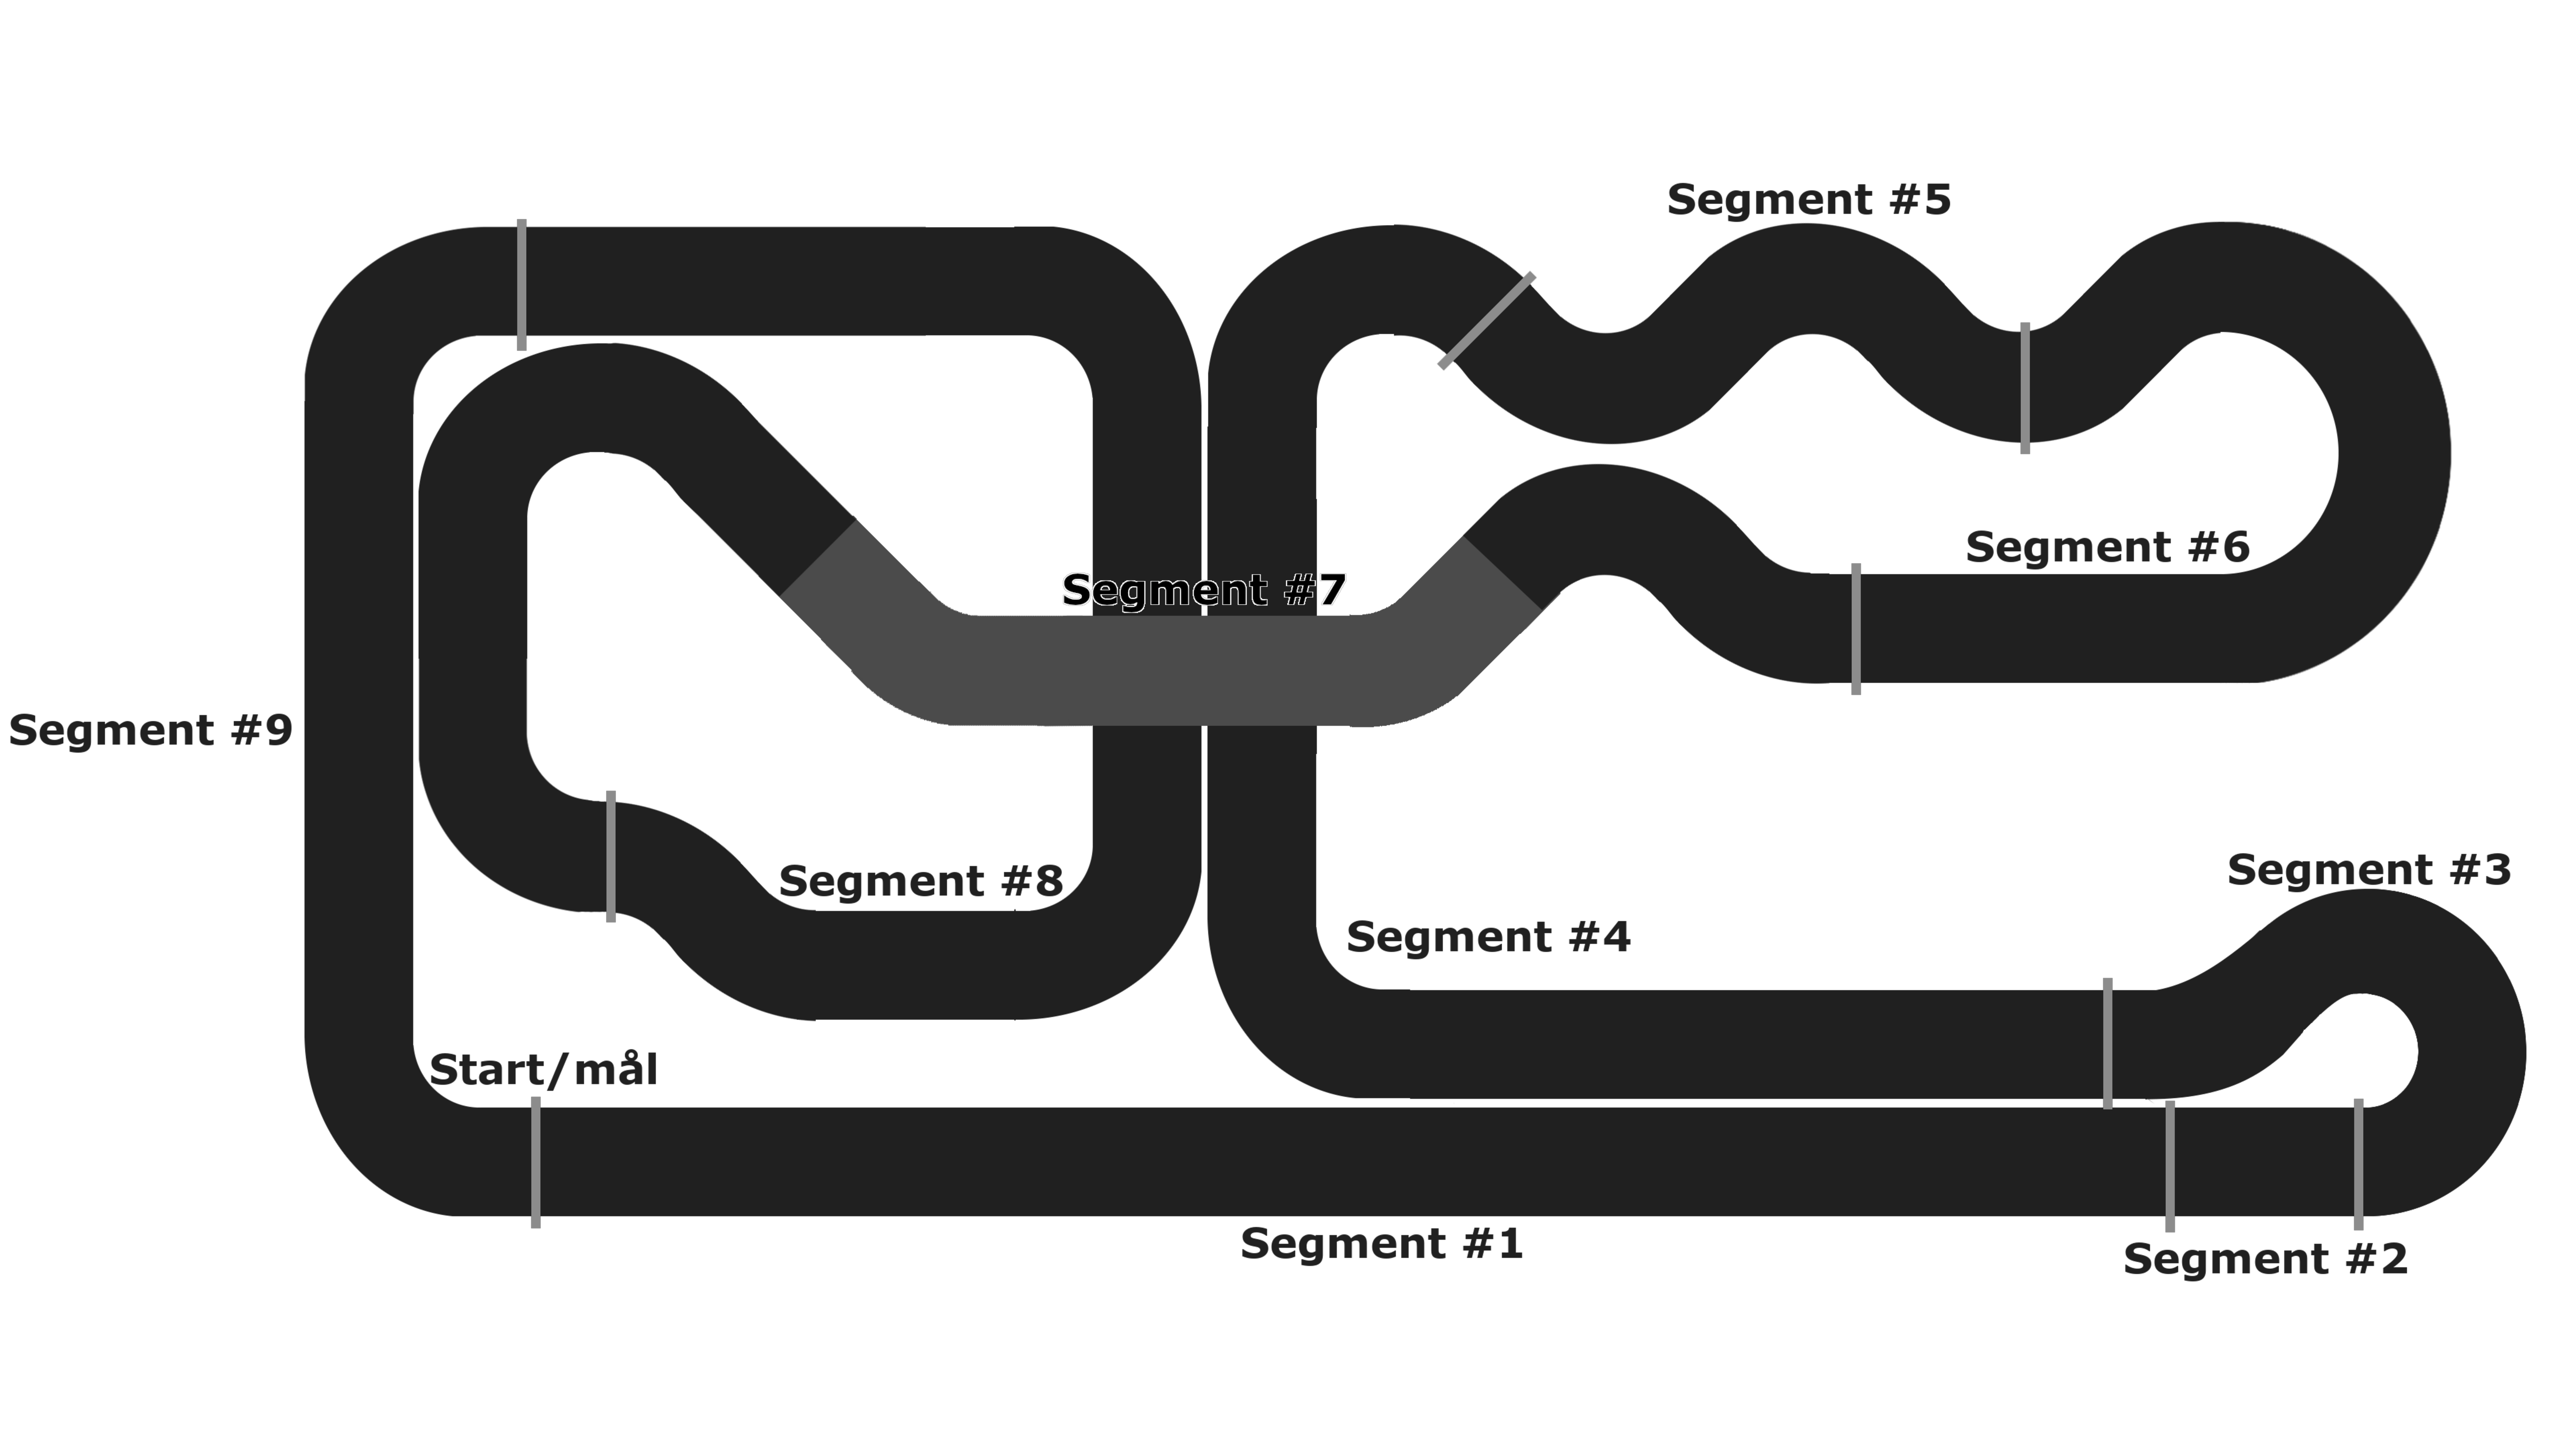
\includegraphics[width=\linewidth] {Figures/BanaModell}
	\caption{En modell av bilbanan.}
	\label{fig:bilbanan}
\end{figure}

\subsection{Bakgrund} 

Projektet har utförts med hjälp av en bilbana samt flera bilar, givare,
spänningsaggregat och två datorer. Via datorn har spänning
tillförts till bilbanan. Med hjälp av givarna är det möjligt att veta när en bil
har passerat en givare. Programvaran har utvecklats i Matlab.

\subsection{Syfte och mål}

Syftet med projektet är att lära sig att arbeta utifrån
projektstyrningsmodellen LIPS. Målet med projektet var att konstruera ett system
som kunde köra bilar runt en bilbana på en vald referenstid mellan 12 och 15
sekunder. Detta skulle göras för flera bilar med olika egenskaper. Fler krav som
ska klaras av finns i kravspecifikationen (\ref{app:kravbeskrivning}).

\subsection{Avgränsningar}

- Ingen gemensam målgång
